\section{Proposed generic architecture}\label{sec:parchitecture}

Currently, the methods of Deep Learning are achieving great results that are revolutionizing the way to address the problems of Artificial Vision, these techniques can solve problems that previously could not be solved, even in some cases surpassing the results presented by a human being, especially in image recognition. End-to-end architectures have the advantage of internally learning features that describe the data in a way to produce an expected result. Nevertheless, they are highly dependant on the dataset variety to be generally applicable. Also, large number of examples is required in most cases to train the networks. A different solution that can cope with those problems, is the use of algorithmic pre-defined features that convert the data to a different known space and train a network with those features. In this way, we detach the motion description from the behaviour classification and allow the system to train ones regardless the specific dataset since we train the network from the features. Since those features are known (i.e. they always have the same shape and range) and not learnt from a specific dataset, and the network learns from them, the generality is implicit regardless the original data. Another advantage of this solution is that a smaller amount of data is required to train the architecture, which is important as not all current datasets have enough images to properly train an end-to-end architecture.

With this idea in mind, the key contribution in this paper is an architecture, depicted in Figure \ref{fig:architecture-general}, that analyses group human behaviour using a movement descriptor and a classification stage to detect different behaviours. For the movement descriptor, in this paper, we present the D-ADV based on the Activity Descriptor Vector (ADV) for deep learning classification, as explained in detail in Section \ref{sec:architecture:DADV}. 

The classification stage is coupled to a learning block as it is shown in Figure \ref{fig:architecture-general}, that classifies the behaviour. There are two main classification strategies, one distinguishes among multiple classes (multi-class classification) and the other between known and unknown behaviours (one-class classification). The second is common in human behaviour as most of the times people act normally, so it is highly unlikely to find enough data to train a network for abnormal activities. Thus, a system is trained to detect the known classes and "classify" the rest as abnormal or unknown. Using a motion descriptor let the system be adaptable to any of these two strategies, that we instantiated after in Section \ref{subsec:arq-occ} for one-class and Section \ref{subsec:arq-mcc} for multi-class.

%Despite the great effort made by the scientific community to improve the automatic analysis of human behaviour, there are still many open challenges. As described above, current proposals for analysing human behaviour are based on integrated deep learning solutions. That is, the same neural network fed directly with the sequence of images of the scene is able to classify it. This is because the network is able to learn, on its own, both the features of the image, or sequence, that best define the solution to the problem, and the network parameters that best separate those features to determine the correct classification. In this way, learning is performed on the whole process, providing very high performances but lacking, in some cases, generality. On the other hand, the results are usually conditioned by the volume of data available: the larger the volume of data, the better the results. In other words, a small dataset does not ensure the goodness of the proposed solutions. Finally, among the current challenges, the lack of generality in current proposals, in terms of the number of individuals in the scene (i.e., from a group of two or more people to crowds), makes it difficult to establish a reference architecture to define how to approach different cases using similar proposals.

%As a scientific contribution to the solution of this type problem, this paper proposes a computer vision architectural model capable of learning and recognising the activities of groups of people using their movements in the scene. The model consists of two main blocks (see Figure \ref{fig:architecture-general}): the local representation of the movement and the classification. In this way, we try to combine the best capabilities of (deep) learning with robust descriptors that allow us to generalise the input data. To this end, it is hypothesised that the use of the appearance of motion in the scene and context could be used to establish an architectural model for solving group activity classification and anomaly detection independently of the number of people involved.

%It has been shown in the state of the art that the use of trajectory descriptors improves the quality of the estimation of the actual behaviour, as it provides a simple and high level of understanding of the activities of complex groups. Therefore, the first block of the model (Fig. \ref{fig:architecture-general}) is able to describe the movement in the scene from local representations of the movement in a region of the scene. It is based on the Activity Descriptor Vector (ADV), a descriptor capable of representing the trajectory information of an image sequence as a collection of the local motions occurring in specific regions of the scene. The ADV \cite{azorin2013, azorin2015} showed a very good performance, independently of the use of different classifiers, in describing activities related to individuals. Also, it demonstrated its predictive capabilities not only to predict behaviour from new inputs, but also to detect behaviour using a portion of the input, to detect in advance the behaviour performed by a person in a \cite{azorin2014predictive} scene. Finally, a variant of ADV was also specified to analyse group behaviour (G-ADV) in \cite{azorin2016} also showing excellent results. The G-ADV is calculated from the trajectory described by the group and by the individuals that form it. Specifically, it uses three different components: the trajectory followed by the group, the coherence of the individual trajectories in the group and, finally, the movement relations between the different groups in the scene.
%The second block of the proposed model (Fig. \ref{fig:architecture-general}) itself allows for a classification of the group's activities. In computer vision research, deep neural networks have evolved to be used consistently due to their good results, as discussed above. Deep learning methods have gained superiority over others in the field of image recognition and classification on single images and sequences, such as LSTM-based action recognition , multi-stream-based architectures for behaviour recognition, skeleton-based for human behaviour recognition, and other similar ones analyzed in \cite{feng2019explorations,jing20173d, ding2016profile}. In this proposal, the architectural model is instantiated to solve the one-class learning problem (D-ADV-OC) for the purpose of detecting abnormal behaviour as well as for multi-activity classification (D-ADV-MC).

%%%%% MOVER A INTRO %%%%%%%%%%%%
%Therefore, the main objective in proposing this type of architecture is to combine the advantages of the ADV for representing activities based on the trajectories of individuals, and the deep learning approach, when necessary, by introducing the description of movement as a variant of the ADV. From this objective, the contribution of this architecture is the improvement of generality and performance in the classification of group activities. In addition, the use of the ADV variant allows training the model using small labelled datasets instead of using large volumes of data. Instead of learning from raw image sequences, using the ADV variant allows the network to learn the features of that descriptor, reducing the solution space.

\begin{figure*}[htbp]
	\begin{center}
		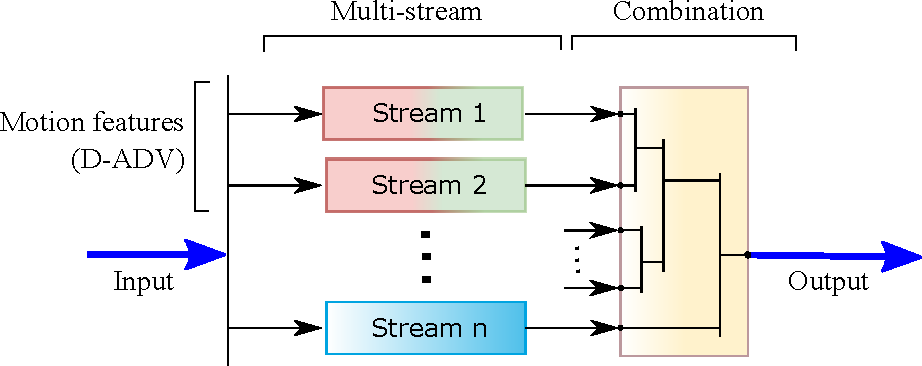
\includegraphics[width=0.6\textwidth]{images/placeholder_figure.pdf}
		\caption[Architectural overview]{Proposed architecture: local movement representation and classification stages.}
		\label{fig:architecture-general}
	\end{center}
\end{figure*}


%\begin{figure*}[htbp]
%	\begin{center}
%		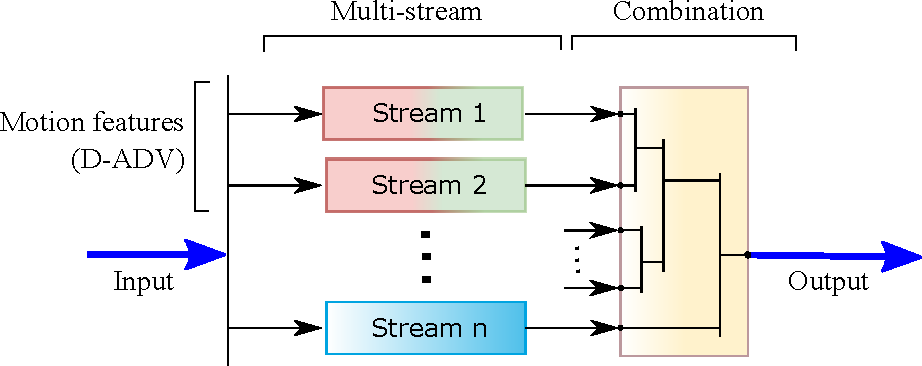
\includegraphics[width=0.7\textwidth]{images/placeholder_figure.pdf}
%		\caption[Architectural overview]{Proposed architecture: local movement representation and classification stages.}
%		\label{fig:architecture-general}
%	\end{center}
%\end{figure*}


%\begin{figure*}[htbp]
%	\begin{center}
%		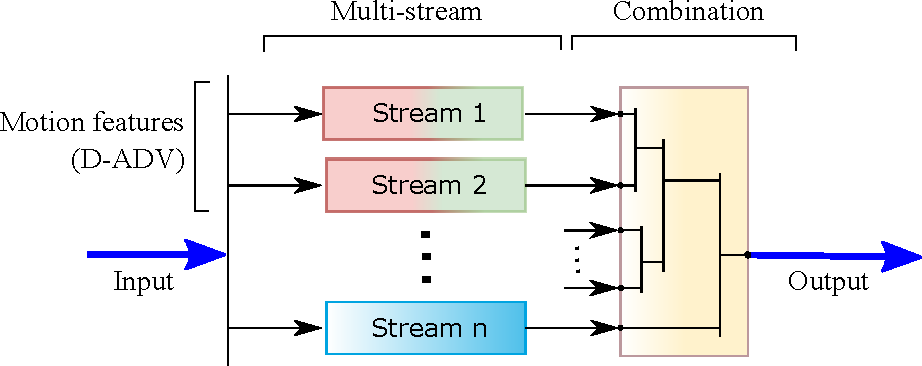
\includegraphics[width=0.7\textwidth]{images/placeholder_figure.pdf}
%		\caption[Overview of two and three streams]{This figure summarises the proposed architecture where the black lines and arrows represent the data flow in two and three streams, on the left side for D-ADV-MC, and on the right side for D-ADV-OC.}
%		\label{fig:two-three-streams}
%	\end{center}
%\end{figure*}




\subsection{Local descriptor motion} \label{sec:architecture:descriptor}

The first block of the architecture aims to extract a representation of the movements that occur in the scene. Here a variant of the ADV descriptor that allows to be used in image-based deep learning systems is presented. Specifically, the Deep-ADV is proposed that allows describing a scene with images of local motions in regions of the scene. For the sake of completeness we first briefly describes the main aspects of the ADV and later the proposed D-ADV. 

\subsubsection{Activity Description Vector (ADV)}\label{sec:architecture:ADV}

The ADV \cite{azorin2013,azorin2015} is a representation of the scene that discretizes the input data into a set of cells where the movement is computed. It has proven good classification capabilities independently of classifiers, in full sequences and in prediction \cite{azorin2014predictive}. G-ADV \cite{azorin2016} is a variant specified to analyse group behaviour. The G-ADV describes the motion of the group and the individuals with three different components: the trajectory of the group, the coherence of the individual in the group and, the movement relations between the different groups in the scene.

The ADV assumes the input data to be a non-perspective set of images (i.e. images on the ground plane), in some cases a pre-process to correct them is required. Using homography (Eq. \ref{eq:Homography}) can help to rectify the data, assuming that any point $p_i$ in the image is transformed into a point $p_g$ in the ground plane $G$.

%consists of a representation method that takes as a reference the scene or terrain where a person moves as a basic geometric model to describe its trajectory considering that the scenario data has no perspective. Therefore, the value space must be perpendicular to the camera focus. In the assumed case that the camera is not located on the ceiling, any information contained in the image plane captured from the static camera must be transformed into the corresponding plane that fits the ground through a homography, H (Eq. \ref{eq:Homography}). The projective transformation allows to consider the whole space of motions of people in a Euclidean space. Then, any point $p_i$ in the image is transformed into a point $p_g$ in the ground plane $G$. 

\begin{equation}\label{eq:Homography}
    p_g = H \cdot p_i
\end{equation}

The ADV uses the information of pairs of consecutive points to find the ratio of movement in the four directions (up, down, left, right, and frequency). Each cell combines the movement information in the descriptor that will later be used to feed a classifier. 
%Since we are only interested in the spatial information of the trajectory to obtain a simple representation to analyze the behavior, the information needed to track the objects in the scene is the position of an individual in the scene. A list of successive $LTP$ points in $G$ is thus established.

%\begin{equation}\label{eq:LTP}
%    LTP = \{p_1,p_2,p_3,\cdots,p_n\}
%\end{equation}


\subsubsection{D-ADV}\label{sec:architecture:DADV}

Deep-ADV (D-ADV) uses apparent motion of the individuals in the scene, in contrast to the original ADV that uses specific movements, i.e. displacement between frames. This gives a more abstract perception of what is happening. In order to do it, a sequence of images is used, and optical flow is calculated from the sequence.  




%This proposal uses a sequence of images as the input set. Unlike ADV, D-ADV does not rely on the specific, individual movements of a person in the scene and the occurrences in the scene (i.e., frequency). It considers the apparent motion of individuals in the visual scene and the appearance of individuals assuming a specific background. For the former, optic flow calculation is the initial stage of the process. It calculates the optical flow between two consecutive frames $(t, t+delta t)$ of the sequence using the differential method as the most commonly used method \cite{KE2018127}. It is based on the assumption of image brightness constancy: given a video sequence, the pixel intensity $(x,y)$ of frame t, $I_t(x,y)$, remains the same despite small changes in position and time period.  If  ($\delta x$,$\delta y$,$\delta t$) is expressed as a small change of motion, and assuming constancy of brightness and expansion as a Taylor series, it can be expressed and approximated as described in \cite{KE2018127}):

%$$ I_{t+\delta t}(x+\delta x, y+\delta y) \approx I_t(x,y) +dato \frac{\partial I}{\partial x}\delta x + \frac{\partial I}{\partial y}\delta y + \frac{\partial I}{\partial t}\delta t $$, solving and dividing the second term along it by $\delta t$, it is possible to obtain:

%$$\frac{\partial I}{\partial x}\frac{\delta x}{\delta t} + \frac{\partial I}{\partial y}\frac{\delta y}{\delta t} + \frac{\partial I}{\partial t} = \frac{\partial I}{\partial x} U + \frac{\partial I}{\partial y} V + \frac{\partial I}{\partial t} \approx 0$$

%where $U = \frac{\delta x}{\delta t}$ y $V = \frac{\delta y}{\delta t}$ are the two components of the optical flow in $t$.

If we assume the image as a ground plane and a static camera (i.e., apparent motion is only generated by the individuals, not by the observer), the difference between two points could be approximated as the derivatives of the pixels  $(p_i - p_{i-1}) \approx (\frac{\delta x}{\delta t},\frac{\delta y}{\delta t}) = (W,V)$. Based on the ADV, we can relate \textit{Up} ($U$) and \textit{Down} ($D$) motion components with vertical $W$ and \textit{Left} ($L$) and \textit{Right} ($R$) with $V$. Hence, the components are calculated as in Eq. \ref{eq:DADV_components}: 

\begin{equation}\label{eq:DADV_components}
    \begin{split}
    & U(I_t)=\left\{\begin{matrix} % "&" sign defines where the split is aligned
        -V_t  &  if \enskip V_t < 0  \\
        0     &  others...
    \end{matrix}
    \right.
    \\
    & D(I_t)=\left\{\begin{matrix} % "&" sign defines where the split is aligned
        V_t &  if \enskip V_t > 0  \\
        0   &  others...
    \end{matrix}
    \right.
    \\
    & L(I_t)=\left\{\begin{matrix} % "&" sign defines where the split is aligned
        -W_t  &  if \enskip W_t < 0  \\
        0     &  others...
    \end{matrix}
    \right.
    \\
    & R(I_t)=\left\{\begin{matrix} % "&" sign defines where the split is aligned
        W_t &  if \enskip W_t > 0  \\
        0   &  others...
    \end{matrix}
    \right.
    \end{split}
\end{equation}
 
The \textit{Frequency} ($F$) refers to the time (frames) in which there are people in the scene regardless if they are moving or not (Eq. \ref{eq:DADV_frequency}):

\begin{equation}\label{eq:DADV_frequency}
    F = | I - B | > 2 \cdot std(I-B),
\end{equation} 

\noindent where $B$ is the background, i.e. an image of the scene with no people. The $std$ refers to the standard deviation, that in this case models the dispersion of the difference between the pixels of the image and the background. In order to reliably estimate the pixels that refer to people, by knowing the variability in the pixels of the background due to camera noise or other interferences, we can robustly define the segmentation threshold with the standard deviation specifically, setting it to twice the $std$. 

Each component of the five is then accumulated over a sequence of frames determined by the accuracy requirements of the problem. An example of the windows size ($ws$) can be seen in Figure \ref{fig:data-flow-ADV}. Then, the accumulated $U$, $D$, $L$, $R$, and $F$, are passed to the classification stage, that is explained in Sec. \ref{sec:architecture:multistream}. In general, the classification stage is proposed to be a multi-stream network architecture. The input of each stream is not a concatenation of the five images, but one with $LRF$ and the other one with $UDF$. In this way, one network takes into account horizontal displacements with the frequency, whilst the other vertical motions with the frequency, isolating the directions to allow the networks to focus better on specific directions. Figure \ref{fig:channels-d-adv} depicts this idea of multi-stream with the $LRF$ and $UDF$ inputs.

%This cumulative stage is responsible for calculating the ADV in a given. On the one hand, the cumulative displacement is responsible for the parameters $L$, $R$, $U$ and $D$, and the first cumulative plane is for the component $F$. The accumulation is considered for a set of consecutive frames. To describe this process graphically, the data flow is explained in figure \ref{fig:data-flow-ADV}.

\begin{figure*}[htbp]
	\begin{center}
		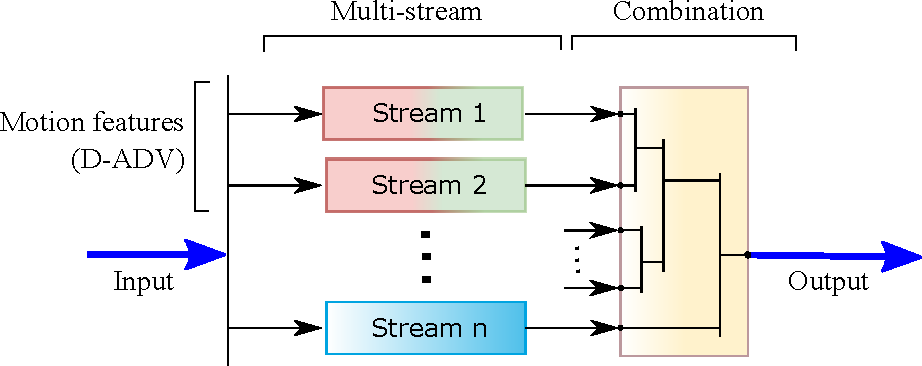
\includegraphics[width=0.95\textwidth]{images/placeholder_figure.pdf}
		\caption[Data stream D-ADV]{Data stream in the image processing stage, where the displacement is calculated and the foreground is extracted from the input image sequence. In the accumulation stage, the displacement and the accumulated frequency are calculated. Continuing with the image classification stage where it receives as input data $LRF$ and $UDF$, to provide the output the different classes of images.}	
		\label{fig:data-flow-ADV}
	\end{center}
\end{figure*}

%Currently, the use of Neural Network architectures for human behavior recognition has become popular. In most cases a single row of layers is used to extract features. However, many authors consider that several networks can be used in parallel, each one specialized in extracting certain features, and once obtained, they can be joined together to improve the hit rate. On this topic there are some works that show the use of several rows of neural networks to detect behaviors \cite{ren2018investigation,ryoo2019assemblenet}. In this paper, a two-row and three-row architecture is proposed: the first and second rows extract the behavioral features according to the movement of people using optical flow, the third row analyzes the scene or context. Figure \ref{fig:two-three-streams} describes in general form the data flow for the D-ADV-OC and D-ADV-MC cases of size $ws$ as shown in figure \ref{fig:name-representation-stage}. The $ws$ parameter is adjusted according to the resulting accuracy requirement, this data indicates the number of images taken from the total sequence as input data to calculate the offset, and then the cumulative offset. In this case, the components are not concatenated all together, they are separated forming two images $LRF$ composed by the components $L$, $R$ and $F$, and, similarly, $UDF$ combines the components $U$, $D$ and $F$. Figure \ref{fig:channels-d-adv} shows separately the images of $LRF$, $UDF$, and the image of a scene of abnormal behavior.

\begin{figure*}[htbp]
	\begin{center}
		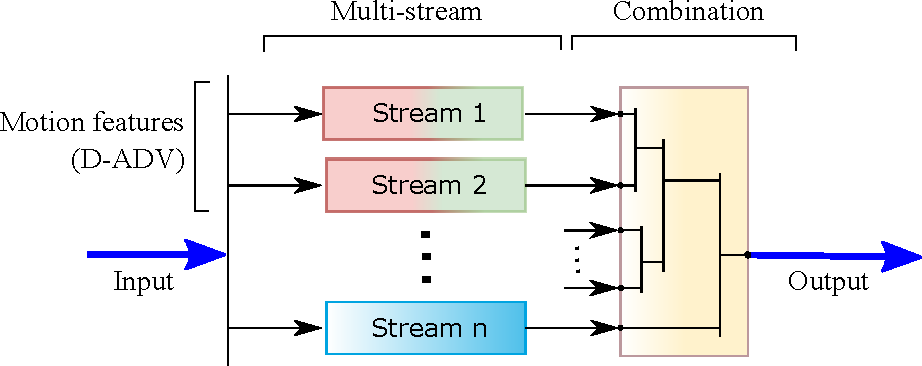
\includegraphics[width=0.7\textwidth]{images/placeholder_figure.pdf}
		\caption[D-ADV rendering stage]{Data flow in the D-ADV-OC rendering stage where the displacement is calculated and foreground is extracted. For the displacement the input is a group of images given by the windowsize ($ws$) parameter, and the output is the accumulated displacement, for the foreground extraction, the input is the background and the output is the accumulated frequency.}	
		\label{fig:name-representation-stage}
	\end{center}
\end{figure*}

\begin{figure}[!h]
	\begin{center}
		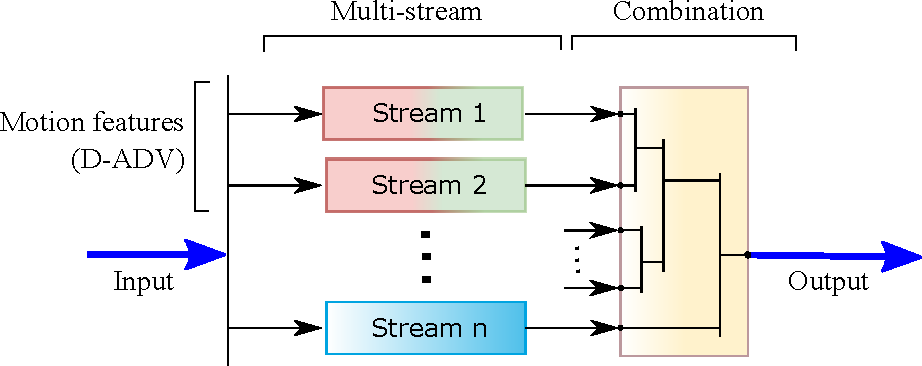
\includegraphics[width=0.5\textwidth]{images/placeholder_figure.pdf}
		\caption[$UDF$, $LRF$, $IMG$ images from D-ADV]{$IMG$, $LRF$, $UDF$ images from D-ADV of an abnormal type behavior scene.}	
		\label{fig:channels-d-adv}
	\end{center}
\end{figure}


\subsection{Classification strategy} \label{sec:architecture:multistream}

%The use of neural network architectures for video sequence analysis has become very popular in recent times. The main idea is to assign a single specific classification task a flow which is usually a network architecture, finding multiple jobs that recognize objects in the scene , locations, fights detection, cancer detection, and many other heterogeneous problems in the field of image classification addressed in the papers \cite{redmon2018yolov3,zalluhoglu2019region,carneiro2019fight}.

The proposed architecture defines, for human behaviour analysis, a classification stage that takes local motion as input and provides a class, either in a range of classes or as a normal/abnormal classification. In the literature review, it has been seen that using multiple networks simultaneously for classification, and fusing their outputs to provide a final decision, achieves better results. This is because each behaviour may have specific features that are learnt by a specific network and then scored, rather than trying to extract all the features within a single global network. This idea is here applied, using a multi-stream strategy, that uses the previously calculated $UDF$ and $RLF$. Also, in some cases, such as in the one-class classification instance of this general architecture (Section \ref{subsec:arq-occ}), another stream can be added for a specific purpose. 

If prediction scores are assigned to each of the network streams (each stream emits scores from different classification tasks), we can weight the features from different points of view. It is very important to efficiently fuse all the streams to generate the final predictions. They can be fused using different methods such as Late fusion (LF), Early fusion (EF), Hybrid fusion (HF) used in \cite{zalluhoglu2019region}. Moreover, a hierarchical fusing can be done that scores two streams that have a common semantic meaning (motion behaviour in the example), and the result is merged with the context stream. 


%A recent trend suggests the combination of some types of architectures in two or more data streams where images or video are input to be analyzed by them in order to extract specific features, classify, etc. and combine their results into a single final classification. In this way, several networks are used in parallel, each one specialized in extracting certain features, and once obtained, they are joined together to improve the hit rate. For example, there are multi-stream architectures that aim to emulate human vision by assuming that the human visual system processes what we see through two types of data streams: the ventral pathway and the dorsal pathway respectively. The ventral pathway is responsible for processing spatial information, such as shape and color, while the dorsal pathway is responsible for processing motion information \cite{kruger2012deep}. To process video sequences and extract features there are proposals to separate the video into spatial and temporal components. The spatial part, as an individual frame, contains information about the scenes and objects found in the video. The temporal part, in the form of movement through frames, conveys the movement of the observer, which in this case is the camera, and the objects in the scene. The spatial and temporal parts of the architecture proposed in \cite{simonyan2014two} are separated into two different data streams. This way of analyzing video sequences is referred to as two-streams architectures, and there are additional works with the same logic of operating two or more data streams \cite{zhu2018hidden,liang2019three}. As for the specific scope of detecting behaviors there are several current works. \cite{ren2018investigation,ryoo2019assemblenet}.

In this paper, the classification stage is proposed (see Figure \ref{fig:name-representation-stage}) to include  of two streams, each related to the D-ADV $UDF$ and $RLF$ descriptors respectively. The combination of both streams is carried out by a final fusion layer that concatenate the stream outputs and pass it to a fully connected layer.  

In addition, the proposed architecture considers, for the case of one-class classification, an extra stream for the context information in the scene. In this case, the fusion of the context stream is done in a weighted way to each of the flows and will depend on the specific application (Figure \ref{fig:contexto-pesos}). 

\begin{figure}[!h]
	\begin{center}
		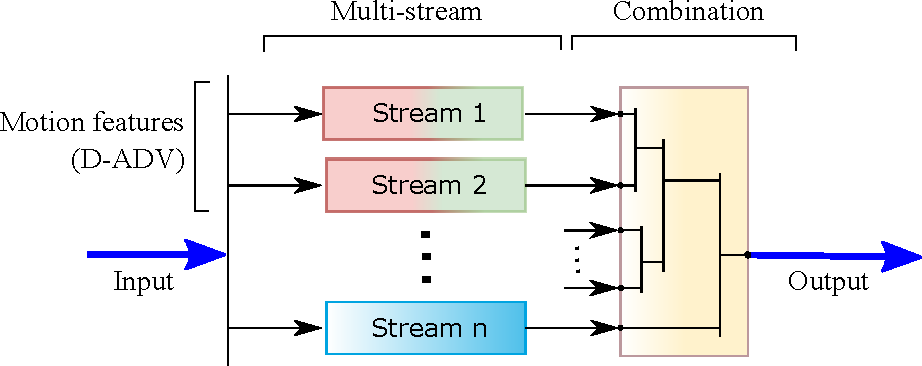
\includegraphics[width=0.5\textwidth]{images/placeholder_figure.pdf}
		\caption[Context recognition block]{As input data to the context recognition block we have a group of images given by the windowsize ($ws$) parameter that are a representative segment of the total number of frames of the analyzed video, the output of this block shows us if the behavior is normal or abnormal.}
		\label{fig:contexto-pesos}
	\end{center}
\end{figure}
